\section{DSL implementation}
The system basically consists out of three parts: a user interface front-end,
a database back-end and an adapter layer between them. The frontend can ask to
execute a query on the database. Then, the appropriate adapter class can make
this
request suitable for the database back-end. It is important to note that
the user-interface only checks for language consistency. For instance it checks
if the primitives are ordered appropriately, but it doesn't check for instance if
a certain country actually exists in the database. The back-end assumes the
entered intermediate code is consistent and only executes the queries. Both
parts are written in \Csh{}. The database part invokes a \texttt{PostgreSQL}
database. Figure \ref{fig:systemOverview} gives a graphical overview of the system.
\begin{figure}[hbt]
\centering
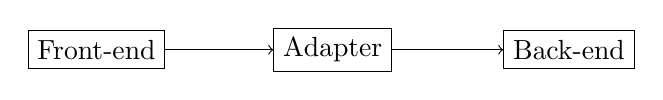
\begin{tikzpicture}
\node[rectangle,draw=black] (F) at (-3,0) {Front-end};
\node[rectangle,draw=black] (A) at (0,0) {Adapter};
\node[rectangle,draw=black] (B) at (3,0) {Back-end};
\draw[->] (F) to node[below]{} (A);
\draw[->] (A) to node[below]{} (B);
\end{tikzpicture}
\caption{Graphical overview of the System}
\label{fig:systemOverview}
\end{figure}
\paragraph{}We will describe each of the parts in detail in the sections below. The code can be found in the directory \texttt{DSLImplementation}.